% Planteamiento del Problema

\chapter{Resumen de actividades} % Chapter title

\label{ch:metodologia} % For referencing the chapter elsewhere, use \autoref{ch:introduction} 
\section{Cronograma}
A continuación se adjunta información referente al las actividades desarrolladas en la primera parte del trabajo.
\begin{center}
    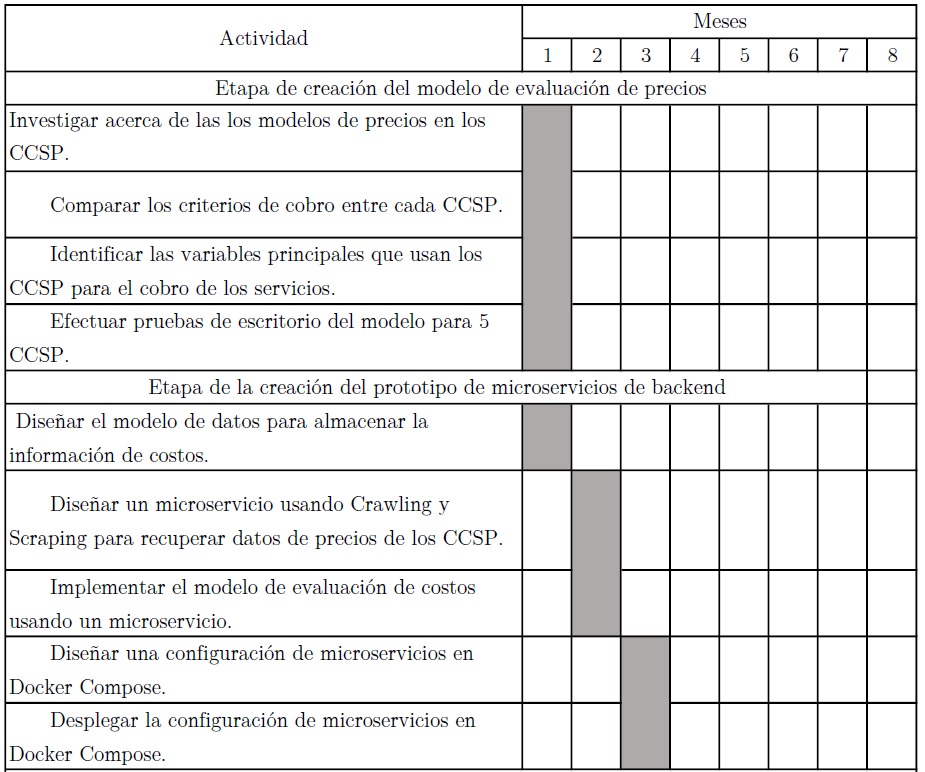
\includegraphics[width=\textwidth]{gfx/actividades.png}
\end{center}

\section{1er Objetivo específico.}
Las actividades de este objetivo específico tienen como propósito \emph{definir un modelo general de evaluación de costos para el análisis de los servicios en el \acrshort{CC} usando información recuperable y relevante de la Web de sus proveedores.} El resultado obtenido son las ecuaciones del modelo de evaluación de costos listas para implementación. A continuación el resumen de cada actividad.

\subsection{Actividades 1 y 2.}
\emph{Investigar acerca de las los modelos de precios en los \acrshortpl{CCSP} y comparar los criterios de cobro entre cada \acrshort{CCSP}:} \newline\newline
Como conclusión de esta actividad y teniendo en cuenta las variables de costo de cada tipo de servicio se formuló el siguiente criterio.

\subsection{Actividad 3.}
\emph{Identificar las variables principales que usan los \acrshortpl{CCSP} para el cobro de los servicios:}
\newline\newline
Como conclusión y resultado de esta actividad se definieron las variables principales que usan los \acrshortpl{CCSP} para el cobro de cada tipo de servicio. Cada variable depende del servicio en cuestión.
\newline\newline

En el caso de el servicios tipo \emph{Compute} y \emph{Container} relacionados con máquinas virtuales y contenedores, la variable de costo principal es el \emph{tiempo de uso} en producto con la \emph{cantidad de CPU's}, la \emph{memoria RAM}.
\newline\newline

Si se habla de un recurso tipo \emph{Storage} y \emph{SQL} la variable de costo principal es el \emph{tamaño de almacenamiento} en producto con la \emph{disponibilidad}, este último se relaciona con lo que será almacenado y cómo será recuperado. (Ej: Archivos, objetos o bases de datos. Modo frio o alta velocidad).
\newline\newline

\subsection{Actividad 4.}
\emph{Efectuar pruebas de escritorio del modelo para 5 \acrshortpl{CCSP}}:
\newline\newline

\section{2do Objetivo específico.}
Las actividades de este objetivo específico tienen como propósito \emph{diseñar e implementar un prototipo basado en microservicios que recopile periodicamente y almacene las tarifas de los principales \acrshortpl{CCSP}}. El resultado obtenido es un Web service que desempeña las tareas mencionadas. A continuación el resumen de cada actividad.

\subsection{Actividad 5.}
\emph{Diseñar el modelo de datos para almacenar la información de costos:}
\newline\newline
Como resultado de esta actividad se diseñó el esquema de la base de datos usando el \acrshort{ORM} \gls{Sequelize} sobre \gls{PostgreSQL}, Los archivos relacionados con cada Entidad de la base de datos se encuentran en \url{https://github.com/sebastianaf/pricecloud/tree/master/api-01/src/db/models}.

\subsection{Actividad 6.}
\emph{Diseñar un microservicio que use técnicas de \emph{Crawling} y \emph{Scraping} para recuperar datos de precios de los \acrshortpl{CCSP}}:
\newline\newline
Como resultado de esta actividad se costruyó el servicio escrito en \emph{Python} ubicado en \url{https://github.com/sebastianaf/pricecloud/tree/master/api-02}. A la fecha de elaboración de este informe se continúa trabajando en recuperar la información de costos en algunos \acrshortpl{CCSP} mencionados en la \emph{sección 1.1}

\subsection{Actividad 7.}
\emph{Implementar el modelo de evaluación de costos usando un microservicio:}\newline\newline
Como resultado de esta actividad se creó el endpoint ubicado en \url{https://api.pricecloud.enerfris.com/evaluate}. El código referente a este endpoint se encuentra en \url{https://api.pricecloud.enerfris.com/evaluate}

\subsection{Actividad 8.}
\emph{Diseñar una configuración de microservicios en \gls{Docker Compose}:}
\newline\newline
 Como resultado de esta actividad se codificó el archivo \emph{docker-compose.yml} ubicado en \url{https://github.com/sebastianaf/pricecloud/blob/master/docker-compose.yml} donde están configurados todos los servicios de la primera parte de la aplicación,

\subsection{Actividad 9.}
\emph{Desplegar la configuración de microservicios en \gls{Docker Compose}:}
\newline\newline
Como resultado de esta actividad se desplegaron tres \acrshortpl{API REST} ejecutando los servicios descritos en la \emph{sección 1.2}.
\newline\newline
Los servicios se encuentran desplegados en las siguientes ubicaciones:
\begin{itemize}
    \item \url{https://pricecloud.enerfris.com}
    \item \url{https://api.pricecloud.enerfris.com}
    \item \url{https://db.pricecloud.enerfris.com}
\end{itemize}


\newpage

%----------------------------------------------------------------------------------------
